\chapter{\label{sec:scandata} Animation of Scanned Data}

In chapter \ref{sec:skeletalanim}, we presented a method of animating a polygon mesh using skeletal motion to drive changes in the geometry of a simple mesh. However, we are ultimately interested in animating extremely dense meshes, rather than the low-detail meshes discussed above. It would be possible to apply the above method directly to such dense data, but such a solution would not satisfy our requirement of interactive control of the animation, as animating a dense mesh directly would require a prohibitive amount of computation. Therefore, we continue with the layered animation approach introduced in chapter \ref{sec:introduction} and use the dense scan data to build a top-level {\it detail layer}.

We require a number of properties for our detail layer surface; firstly, it must be defined in terms of the control layer so that it can be animated by deformations of that layer. Secondly, these animations should be smooth and seamless; they should not introduce cracks or discontinuities that were not present in the original data.

In order to redefine the detail layer in terms of the control layer, we need to define a mapping from a volume to a 2D surface, as the control layer is a 2D surface embedded in ${\mathbb R}^3$. The mapping should be continuous across the space, with no sharp boundaries. It should also be capable of smooth animation, so that the space deforms smoothly as the control layer moves. We also require this mapping to be invertible, as we wish to both perform a mapping of the detail layer to the control layer, and also the inverse, i.e. reconstruction of the detail layer surface. The mapping function must therefore be bijective in our region of interest.

We perform this mapping using a {\it normal volume} approach, which is similar to the skeletal mapping method described above, in that it defines a point in space in terms of a point on a known surface, plus an offset along a normal vector. This formulation allows us to represent a detailed mesh in terms of a simpler one, and to smoothly animate the two meshes together.

\section{\label{sec:scandata:normalvolume}The Normal Volume}
\nomenclature{\bf Normal Volume}{A volumetric envelope which extends above and below a triangle surface, whose boundaries are defined by the normals at the triangle vertices.}
\begin{figure}
\begin{center}
\setlength{\unitlength}{0.4cm}
\begin{picture}(21,11)
% M
\thicklines
\put(2,4){\circle*{0.2}}
\put(2,4){\line(4,3){4}}
\put(6,7){\circle*{0.2}}
\put(6,7){\line(4,-1){4}}
\put(10,6){\circle*{0.2}}
\put(10,6){\line(1,0){4}}
\put(14,6){\circle*{0.2}}
\put(14,6){\line(2,-1){4}}
\put(18,4){\circle*{0.2}}
% M+
\put(1,8){\line(4,3){4}}
\put(5,11){\line(6,-1){6}}
\put(11,10){\line(1,0){4}}
\put(15,10){\line(5,-2){5}}
% M-
\put(3,0){\line(4,3){4}}
\put(7,3){\line(2,-1){2}}
\put(9,2){\line(1,0){4}}
\put(13,2){\line(3,-2){3}}
% Normals
\thinlines
\put(3,0){\vector(-1,4){2}}
\put(7,3){\vector(-1,4){2}}
\put(9,2){\vector(1,4){2}}
\put(13,2){\vector(1,4){2}}
\put(16,0){\vector(1,2){4}}
% Labels
\put(2,0){$\vec{v}_x^-$}
\put(1,4){$\vec{v}_x$}
\put(0,8){$\vec{v}_x^+$}
\put(1.5,6.5){$\vec{n}_x$}
\put(17,0){$M^-$}
\put(19,4){$M$}
\put(21,8){$M^+$}
\end{picture}
\caption[Offset Surfaces]{\label{fig:offsetsurface} Offset surface of a mesh. The two offset surfaces $M^+$ and $M^-$ define a volumetric envelope around $M$.}
\end{center}
\end{figure}

In order to perform this mapping, we use the concept of the normal volume or {\it fundamental prism}, introduced by \citet{Cohen96} and which was extended by Adrian Hilton in \cite{Sun01}. We first create a volumetric envelope, which is defined over the mesh $M$ that we want to map to, and which completely encloses it. This envelope is formed by taking each vertex $\vec{v}_x \in {\cal V}_M$ and translating it along its normal vector $\vec{n}_x$ by two distances $d^+$ and $d^-$, creating two new points, ${\vec{v}_x}^+$ and ${\vec{v}_x}^-$, as shown in figure \ref{fig:offsetsurface}. This defines two offset surfaces, $M^+$ and $M^-$.
\begin{eqnarray}
\vec{v}_x^+ & = & \vec{v}_x + d^+\vec{n}_x \\
\vec{v}_x^- & = & \vec{v}_x + d^-\vec{n}_x
\end{eqnarray}

\begin{figure}
\begin{center}
\setlength{\unitlength}{0.5cm}
\begin{tabular}{cc}
\begin{picture}(13,14)
% triangles
\thicklines
\put(5,1){\line(2,1){2}}
\put(5,1){\line(3,-1){3}}
\put(7,2){\line(1,-2){1}}
\put(3,6){\line(2,1){4}}
\put(3,6){\line(3,-1){6}}
\put(7,8){\line(1,-2){2}}
\put(1,11){\line(2,1){6}}
\put(1,11){\line(3,-1){9}}
\put(7,14){\line(1,-2){3}}
% points
\put(5,1){\circle*{0.2}}
\put(7,2){\circle*{0.2}}
\put(8,0){\circle*{0.2}}
\put(3,6){\circle*{0.2}}
\put(7,8){\circle*{0.2}}
\put(9,4){\circle*{0.2}}
\put(1,11){\circle*{0.2}}
\put(7,14){\circle*{0.2}}
\put(10,8){\circle*{0.2}}
% normals
\thinlines
\put(5,1){\line(-2,5){4}}
\put(7,2){\line(0,1){12}}
\put(8,0){\line(1,4){2}}
% vertex labels
\put(4,0.5){$\vec{v}_a^-$}
%\put(7.5,2){$\vec{v}_b^-$}
%\put(8.5,0){$\vec{v}_c^-$}
\put(2,5.5){$\vec{v}_a$}
%\put(7.5,7){$\vec{v}_b$}
%\put(9.5,3){$\vec{v}_c$}
\put(0,10.5){$\vec{v}_a^+$}
%\put(7.5,12){$\vec{v}_b^+$}
%\put(10.5,6){$\vec{v}_c^+$}
% normal labels
\put(2.5,8){$\hat{n}_a$}
%\put(6,9){$\vec{n}_b$}
%\put(8.8,5){$\vec{n}_c$}
% triangle labels
\put(11,1){$t_x^-$}
\put(11,5){$t_x$}
\put(11,11){$t_x^+$}
\end{picture} &
\begin{picture}(13,14)
% triangles
\thicklines
\put(5,1){\line(2,1){2}}
\put(5,1){\line(3,-1){3}}
\put(7,2){\line(1,-2){1}}
\put(7,2){\line(2,-1){2}}
\put(8,0){\line(1,1){1}}
\put(3,6){\line(2,1){4}}
\put(3,6){\line(3,-1){6}}
\put(7,8){\line(1,-2){2}}
\put(7,8){\line(2,-1){4}}
\put(9,4){\line(1,1){2}}
\put(1,11){\line(2,1){6}}
\put(1,11){\line(3,-1){9}}
\put(7,14){\line(1,-2){3}}
\put(7,14){\line(2,-1){6}}
\put(10,8){\line(1,1){3}}
% points
\put(5,1){\circle*{0.2}}
\put(7,2){\circle*{0.2}}
\put(8,0){\circle*{0.2}}
\put(9,1){\circle*{0.2}}
\put(3,6){\circle*{0.2}}
\put(7,8){\circle*{0.2}}
\put(9,4){\circle*{0.2}}
\put(11,6){\circle*{0.2}}
\put(1,11){\circle*{0.2}}
\put(7,14){\circle*{0.2}}
\put(10,8){\circle*{0.2}}
\put(13,11){\circle*{0.2}}
% normals
\thinlines
\put(5,1){\line(-2,5){4}}
\put(7,2){\line(0,1){12}}
\put(8,0){\line(1,4){2}}
\put(9,1){\line(2,5){4}}
\end{picture} \\
{\it (a)} & {\it (b)}
\end{tabular}
\caption[The Normal Volume]{\label{fig:normalvolume} The Normal Volume. (a) The normal volume of a single triangle $t_x$. (b) Adjacent normal volumes form a continuous envelope.}
\end{center}
\end{figure}

As a triangle is made up of a triplet of mesh vertices $t_x\symbol{triangle} = [\vec{v}_a,\vec{v}_b,\vec{v}_c]$, each triangle $t_x \in {\cal T}$ will therefore have a corresponding pair of offset triangles, ${t_x}^+$ and ${t_x}^-$, as illustrated in figure \ref{fig:normalvolume}a. The volume contained within this prism is called the normal volume of the triangle $t_x$, $N_x$\symbol{nv}. The normal volume can also be defined as the union of all offset polygons $t_x^d$ at distance $d$, for $d^- \leq d \leq d^+$.
\begin{eqnarray}
t_x^d & = & [\vec{v}_a^d,\vec{v}_b^d,\vec{v}_c^d] \\
N_x & = & \bigcup^{d^+}_{d=d^-} t_x^d
\end{eqnarray}
The union of all normal volumes ${\cal N}$\symbol{nvset} (see equation \ref{eqn:nvset}) defines a volumetric envelope which encloses the original mesh $M$, and each point $p$ within this envelope lies within a particular normal volume $N_x$, which has a related triangle $t_x$. Therefore, as long as the detail layer mesh ${\cal T_D}$ of our model is wholly contained within the volumetric envelope of the control layer ${\cal N_C}$, each vertex in the detail layer mesh $\vec{v}_x \in {\cal V_D}$ can be associated with a control layer triangle $t_x$.

\begin{equation} \label{eqn:nvset}
{\cal N} = \bigcup^{n-1}_{x=0} N_x
\end{equation}

\subsection{\label{sec:scandata:normalvolume:interpolation}Normal Interpolation}

\begin{figure}
\begin{center}
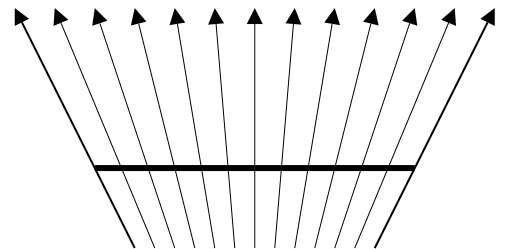
\includegraphics[width=7cm]{../images/normals}
\caption[Normal Interpolation]{\label{fig:normalinterpolation} Normal Interpolation. A slice through a normal volume, showing how triangle normals are interpolated across the surface of the associated triangle.}
\end{center}
\end{figure}

A planar polygon in 3D space has a single normal vector, which is perpendicular to the polygon surface. In a polygon mesh, however, each vertex also has a normal vector, defined as a combination of the surrounding face normals. In our normal volume representation, however, a single triangle does not have a single normal. Each point on the triangle surface will have a unique normal value, as shown in figure \ref{fig:normalinterpolation}. 

The normals are linearly interpolated across the surface of the triangle, and the normal $\vec{n}_j$ at any point $p_j$ on the triangle surface can be expressed as a linear combination of the three vertex normals:

\begin{equation} \label{eqn:interpolatednormals}
\vec{n}_j = \omega_a\hat{n}_a + \omega_b\hat{n}_b + \omega_c\hat{n}_c
\end{equation}

Where $\hat{n}_x\symbol{normal}$ is the surface normal at the vertex $\vec{v}_x$, and $\omega_x$ is an areal coordinate component for that point and vertex, as described below in section \ref{sec:scandata:pointtosurface:areal}. This kind of normal interpolation technique is often used in Phong shading of polygon meshes \cite{Phong75}. 

\subsection{\label{sec:scandata:normalvolume:collapse}Normal Volume Collapse}

\begin{figure}
\begin{center}
\setlength{\unitlength}{0.5cm}
\begin{picture}(9,12)
% triangles
\thicklines
\put(8,1){\line(-2,-1){2}}
\put(8,1){\line(-3,1){3}}
\put(6,0){\line(-1,2){1}}
\put(4,5){\line(2,1){2}}
\put(4,5){\line(3,-1){3}}
\put(6,6){\line(1,-2){1}}
\put(0,9){\line(2,1){6}}
\put(0,9){\line(3,-1){9}}
\put(6,12){\line(1,-2){3}}
% points
\put(8,1){\circle*{0.2}}
\put(6,0){\circle*{0.2}}
\put(5,2){\circle*{0.2}}
\put(4,5){\circle*{0.2}}
\put(6,6){\circle*{0.2}}
\put(7,4){\circle*{0.2}}
\put(0,9){\circle*{0.2}}
\put(6,12){\circle*{0.2}}
\put(9,6){\circle*{0.2}}
% normals
\thinlines
\put(4,5){\line(1,-1){4}}
\put(4,5){\vector(-1,1){4}}
\put(6,6){\line(0,-1){6}}
\put(6,6){\vector(0,1){6}}
\put(7,4){\line(-1,-1){2}}
\put(7,4){\vector(1,1){2}}
% triangle labels
\put(9,1){$t_x^-$}
\put(9,4){$t_x$}
\put(9,9){$t_x^+$}
\end{picture}
\caption[Normal Volume Collapse]{\label{fig:normalvolumecollapse} Collapse of the Normal Volume. Under the correct circumstances, the boundaries of a normal volume can intersect.}
\end{center}
\end{figure}

If $d^+$ and $d^-$ are large enough, and the surface is non-planar in some areas, the boundaries of some normal volumes in ${\cal N}$ will start to intersect each other. Figure \ref{fig:normalvolumecollapse} illustrates this situation. The normals are at a steeper angle than in figure \ref{fig:normalvolume}a, and the triangle $t^-$ is below the point at which the boundaries intersect. In the area of the intersection, the mapping from volume to surface is no longer valid, and in the region beyond the collapse, although the mapping is once again valid, it may lead to undesirable results.

Collapse will happen to almost all normal volumes at some point; however, by correct design of the control mesh and correct choice of $d^+$ and $d^-$, we can avoid these situations. There are two properties we must enforce during design of the control layer. The error between the control and detail layers must always be within the range $d^+$ to $d^-$; however, this range must be small enough that collapses can not occur. The process of control layer creation is discussed in detail in section \ref{sec:scandata:creation:control}, along with methods of enforcing the above properties.

\subsection{\label{sec:scandata:normalvolume:boundaries}Boundaries}

\begin{figure}
\begin{center}
\begin{tabular}{ccc}
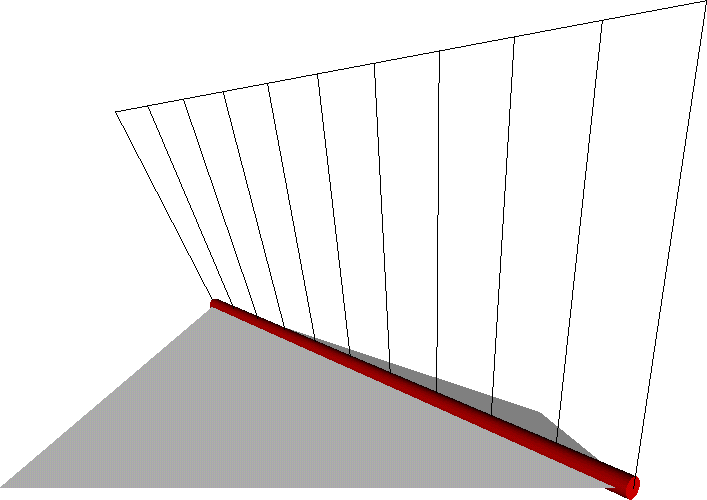
\includegraphics[height=4cm]{../images/ruled_surface_a} &
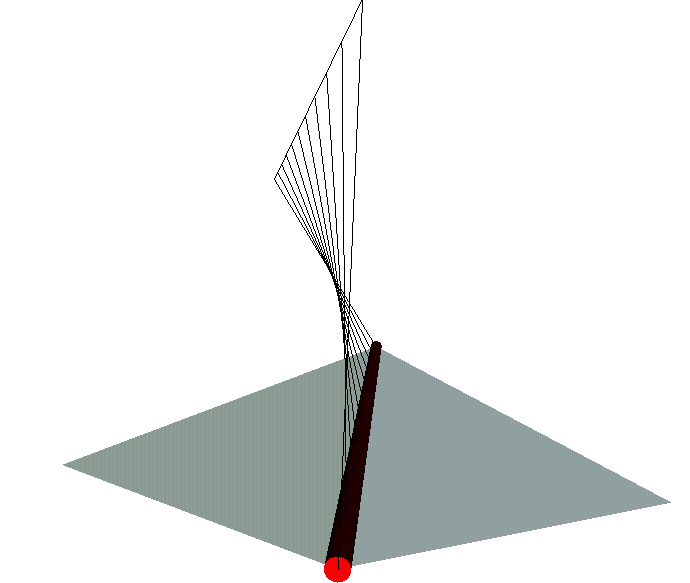
\includegraphics[height=4cm]{../images/ruled_surface_b} &
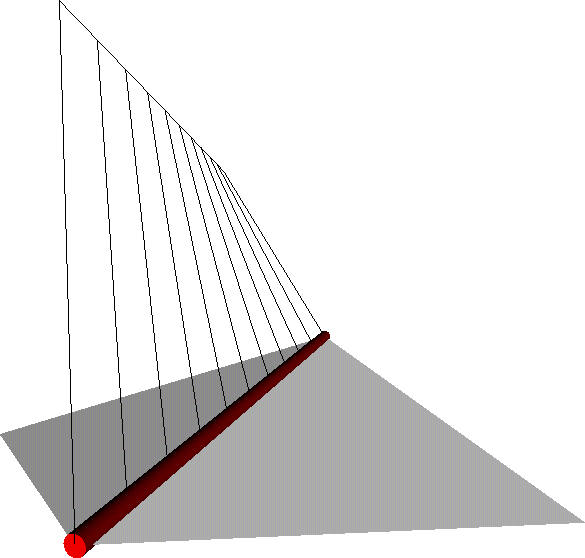
\includegraphics[height=4cm]{../images/ruled_surface_c}
\end{tabular}
\caption[Normal Volume Boundaries]{\label{fig:twistednormals} Normal Volume Boundaries. The boundary of two normal volumes is not planar, but a bilinear ruled surface.}
\end{center}
\end{figure}

It should be noted that the boundaries of a normal volume are not planar. As the boundary is formed by a linear interpolation of the normals at either end, which do not necessarily lie in the same plane, the boundary is in fact a bilinear ruled surface, as shown in figure \ref{fig:twistednormals}. This property does not affect our use of the normal volume at this stage, but will be of importance later on.

\section{\label{sec:scandata:pointtosurface}Point To Surface Mapping}

Once we have defined a volumetric envelope around our mesh surface $M$, we need to define a bijective mapping between an arbitrary point $p$ inside the envelope, and the surface itself. We therefore define a mapping between any point that lies within a normal volume $N_x$, and the related triangle surface $t_x$.

\subsection{\label{sec:scandata:pointtosurface:areal}Areal Coordinates}

\nomenclature{\bf Areal Coordinates}{A coordinate for a point defined by its relation to three or more other points. Each component of the coordinate is a {\it weight} for the corresponding point. The sum of the components is 1.}
Any point $\vec{p}_j \in {\mathbb R}^3$ can be represented as an affine combination of three or more linearly independent points $\vec{p}_0, \vec{p}_1, ..., \vec{p}_n$.

\begin{equation} \label{eqn:barycentric}
\vec{p}_j = \omega_0\vec{p}_0 + \omega_1\vec{p}_1 + ... + \omega_n\vec{p}_n
\end{equation}

The coefficients $(\omega_0, \omega_1, ..., \omega_n)\symbol{areal}$ make up a {\it barycentric coordinate}. Barycentric coordinates are in fact a general form of this type of coordinate, and in the case where the sum of all $\omega_i$ is 1, they are called {\it areal coordinates} \cite{Weisstein99}. If all points $\vec{p}_i$ are coplanar, the resulting point $\vec{p}_j$ will also lie on that plane. This allows us to represent any point $\vec{p}_j$ on the surface of a triangle $t_x$ in this form, by defining an areal coordinate for the point in terms of the triangle vertices $(\vec{v}_a,\vec{v}_b,\vec{v}_c)$.

\begin{equation} \label{eqn:interpolatedpoint}
\vec{p}_j = \omega_a\vec{v}_a + \omega_b\vec{v}_b + \omega_c\vec{v}_c
\end{equation}

\begin{figure}
\begin{center}
\setlength{\unitlength}{0.4cm}
\begin{picture}(20,12)
% triangles
\thicklines
\put(1,6){\line(2,1){12}}
\put(1,6){\line(3,-1){18}}
\put(13,12){\line(1,-2){6}}
% points
\put(1,6){\circle*{0.2}}
\put(13,12){\circle*{0.2}}
\put(19,0){\circle*{0.2}}
\put(11,6){\circle*{0.2}}
% internal lines
\thinlines
\put(1,6){\line(5,0){10}}
\put(13,12){\line(-1,-3){2}}
\put(19,0){\line(-4,3){8}}
% labels
\put(0,6){$\vec{v}_a$}
\put(13.5,12){$\vec{v}_b$}
\put(19.5,0){$\vec{v}_c$}
\put(12,6){$\vec{p}_j$}
\put(14,6){$\omega_a$}
\put(10,4){$\omega_b$}
\put(9,8){$\omega_c$}
\put(2,1){$\omega_a + \omega_b + \omega_c = 1$}
\end{picture}
\caption[Areal Coordinates]{\label{fig:arearatios} Areal coordinates are calculated from area ratios of each sub-triangle and the enclosing triangle.}
\end{center}
\end{figure}

Such an areal coordinate is normally calculated by the use of area ratios, as shown in figure \ref{fig:arearatios}. $\omega_i$ is equal to the ratio of the area of the triangle opposite the vertex to the area of the entire triangle, and can be calculated using the 2D cross product method shown in the following equations.
\begin{eqnarray}
{\cal A} & = & (\vec{v}_b - \vec{v}_a) \times (\vec{v}_c - \vec{v}_a) \\
\omega_a & = & ((\vec{v}_b - \vec{p}_j) \times (\vec{v}_c - \vec{p}_j)) / {\cal A} \\
\omega_b & = & ((\vec{p}_j - \vec{u}_a) \times (\vec{v}_c - \vec{v}_a)) / {\cal A} \\
\omega_c & = & ((\vec{v}_b - \vec{u}_a) \times (\vec{p}_j - \vec{v}_a)) / {\cal A}
\end{eqnarray}

\subsection{\label{sec:scandata:pointtosurface:nvmapping}Normal Volume Mapping}

As the normal volume $N_x$ is defined based on the vertex positions and normals of the triangle $t_x$, any point $\vec{p}_x$ inside the normal volume $N_x$ can be represented as a combination of a point on the surface of the triangle and a multiple $d$\symbol{distance} of the interpolated normal at that point. Combining equations \ref{eqn:interpolatedpoint} and \ref{eqn:interpolatednormals}:
\begin{eqnarray} \label{eqn:pointinvolume}
\vec{p}_x & = & \vec{p}_j + d \vec{n}_j\nonumber \\
          & = & \omega_a\vec{v}_a + \omega_b\vec{v}_b + \omega_c\vec{v}_c + d(\omega_a\hat{n}_a+\omega_b\hat{n}_b+\omega_c\hat{n}_c)
\end{eqnarray}

In order to be able to express a point inside the normal volume $N_x$ in terms of the triangle $t_x$, we therefore calculate the parameters $\omega_a$, $\omega_b$, $\omega_c$ and $d$ for that point. We first define some useful symbols which will aid our derivation.
\begin{eqnarray} \label{eqn:pointsymbols}
\vec{p}_a & = & \vec{v}_a + d\hat{n}_a \nonumber \\
\vec{p}_b & = & \vec{v}_b + d\hat{n}_b \nonumber \\
\vec{p}_c & = & \vec{v}_c + d\hat{n}_c
\end{eqnarray}

Rearranging and rewriting equation \ref{eqn:pointinvolume} in these terms, we have

\begin{equation}
\vec{p}_x = \omega_a\vec{p}_a + \omega_b\vec{p}_b + \omega_c\vec{p}_c
\end{equation}

However, as noted above, $\omega_a + \omega_b + \omega_c = 1$, so we can remove $\omega_c$ from our representation for good, from now on implicitly defining it in terms of the two remaining $\omega$ components.
\begin{eqnarray} \label{eqn:nomoreomegat}
\omega_c & = & 1 - \omega_a - \omega_b \nonumber \\
\vec{p}_x & = & \omega_a\vec{p}_a + \omega_b\vec{p}_b + (1-\omega_a-\omega_b)\vec{p}_c
\end{eqnarray}
This leaves us with a representation in which we can represent any point inside the normal volume $N_x$ using just three components: $\omega_a$, $\omega_b$ and $d$. These are the parameters we need to compute in order to perform our mapping.

\subsection{\label{sec:scandata:pointtosurface:mappingsoln}Mapping Solution}

We can now solve equation \ref{eqn:nomoreomegat} for the three unknown components, $\omega_a$, $\omega_b$ and $d$. We first rearrange, and use the fact that $\vec{a} \times \vec{a} = \vec{0}$ to remove the $\omega_b$ component.
\begin{eqnarray} \label{eqn:pointonplane}
\vec{p}_x-\vec{p}_c & = & \omega_a(\vec{p}_a-\vec{p}_c) + \omega_b(\vec{p}_b-\vec{p}_c) \nonumber \\
(\vec{p}_x-\vec{p}_c) \times (\vec{p}_b-\vec{p}_c) & = & \omega_a((\vec{p}_a-\vec{p}_c) \times (\vec{p}_b-\vec{p}_c))
\end{eqnarray}
\begin{figure}
\begin{center}
\setlength{\unitlength}{0.8cm}
\begin{picture}(10,9)
% triangles
\thicklines
\put(3,2){\line(2,1){4}}
\put(3,2){\line(3,-1){6}}
\put(7,4){\line(1,-2){2}}
\put(1,6){\line(2,1){6}}
\put(1,6){\line(3,-1){9}}
\put(7,9){\line(1,-2){3}}
% points
\put(3,2){\circle*{0.2}}
\put(7,4){\circle*{0.2}}
\put(9,0){\circle*{0.2}}
\put(1,6){\circle*{0.2}}
\put(7,9){\circle*{0.2}}
\put(10,3){\circle*{0.2}}
\put(6,2){\circle*{0.2}}
\put(5,6){\circle*{0.2}}
% normals
\thinlines
\put(3,2){\vector(-1,2){2}}
\put(7,4){\vector(0,1){5}}
\put(9,0){\vector(1,3){1}}
\put(6,2){\vector(-1,4){1}}
% lines
\put(3,2){\line(1,0){3}}
\put(7,4){\line(-1,-2){1}}
\put(9,0){\line(-3,2){3}}
% vertex labels
\put(2,1.5){$\vec{v}_a$}
\put(1,3.5){$d\hat{n}_a$}
\put(0,5.5){$\vec{p}_a$}
\put(6.5,2){$\vec{p}_j$}
\put(5.5,6){$\vec{p}_x$}
\end{picture}
\caption[Normal volume and point-to-surface mapping]{\label{fig:pointtosurface} Normal volume mapping. A point is mapped onto a single triangle.}
\end{center}
\end{figure}
This equation shows that the point $\vec{p}_x$ lies on a plane formed by the three points $\vec{p}_a$, $\vec{p}_b$, and $\vec{p}_c$, as illustrated in figure \ref{fig:pointtosurface}. The left hand side of the equation is equivalent to twice the area of the triangle formed by $\vec{p}_x$, $\vec{p}_b$, and $\vec{p}_c$. The right hand side is twice the area of the original triangle, scaled by the areal coordinate $\omega_a$. The linear relationship between the two areas will hold true for all cases where the four points are coplanar.

We can now use the fact that $(\vec{a} \times \vec{b}) \cdot \vec{a} = 0$ to remove the $\omega_a$ component and leave us with an equation in which the only unknown is $d$.

\begin{equation}
((\vec{p}_x-\vec{p}_c) \times (\vec{p}_b-\vec{p}_c)) \cdot (\vec{p}_a-\vec{p}_c) = 0
\end{equation}

We then expand this, substituting back in equations \ref{eqn:pointsymbols}.
\begin{eqnarray}
((\vec{p}_x-(\vec{v}_c + d\hat{n}_c)) \times ((\vec{v}_b + d\hat{n}_b)-(\vec{v}_c + d\hat{n}_c))) & \cdot & \nonumber \\
((\vec{v}_a + d\hat{n}_a)-(\vec{v}_c + d\hat{n}_c)) & = & 0
\end{eqnarray}

This equation can then be rearranged into a cubic equation in $d$:
\begin{eqnarray} \label{eqn:cubicd}
d^3((\hat{n}_c \times \hat{n}_b) \cdot \hat{n}_a) & + & \nonumber \\
d^2((\hat{n}_c\times \hat{n}_b )\cdot \vec{v}_a + (\hat{n}_c\times \vec{v}_b )\cdot \hat{n}_a & + & \nonumber \\
(\vec{v}_c\times \hat{n}_b)\cdot \hat{n}_a - ((\hat{n}_a - \hat{n}_c)\times(\hat{n}_a - \hat{n}_b))\cdot \vec{p}_x) & + & \nonumber \\
d((\hat{n}_c\times \vec{v}_b)\cdot \vec{v}_a + (\vec{v}_c\times \hat{n}_b)\cdot \vec{v}_a & + & \nonumber \\
(\vec{v}_c\times \vec{v}_b)\cdot \hat{n}_a - ((\hat{n}_a - \hat{n}_c)\times(\vec{v}_a - \vec{v}_b))\cdot \vec{p}_x & - & \nonumber \\
((\vec{v}_a - \vec{v}_c)\times(\hat{n}_a - \hat{n}_b))\cdot \vec{p}_x) & + & \nonumber \\
(\vec{v}_c\times \vec{v}_b)\cdot \vec{v}_a - ((\vec{v}_a - \vec{v}_c)\times(\vec{v}_a - \vec{v}_b))\cdot \vec{p}_x & = & 0
\end{eqnarray}
The roots of this equation can be found using standard methods. Real values of $d$ correspond to potential planes in which the point $\vec{p}_x$ lies. By calculating the $\omega$ coordinates, we can determine which of these planes gives the correct result. Once we have obtained a value for $d$, then we can rearrange equation \ref{eqn:pointonplane} to calculate the corresponding value for $\omega_a$: 

\begin{equation} \label{eqn:omega_a}
\omega_a = \frac{((\vec{p}_x-\vec{p}_c) \times (\vec{p}_b-\vec{p}_c)) \cdot ((\vec{p}_a-\vec{p}_c) \times (\vec{p}_b-\vec{p}_c))}{\|(\vec{p}_a-\vec{p}_c) \times (\vec{p}_b-\vec{p}_c)\|^2}
\end{equation}

We can then rearrange equation \ref{eqn:nomoreomegat} to give us a value for $\omega_b$, completing our parameterisation.

\begin{equation} \label{eqn:omega_b}
\omega_b = \frac{(\vec{p}_x - \vec{p}_c - \omega_a(\vec{p}_a - \vec{p}_c)) \cdot (\vec{p}_b-\vec{p}_c)}{\|(\vec{p}_b-\vec{p}_c)\|^2}
\end{equation}

There may be more than one potential value of $d$ for a mapping, however there should only be one result which gives valid values for $\omega_a$ and $\omega_b$. As the areal coordinates for the point $\vec{p}_j$ should sum to 1, valid results are those which satisfy the following criteria.
\begin{eqnarray}
0 \leq & \omega_a & \leq 1 \nonumber \\
0 \leq & \omega_b & \leq 1 \nonumber \\
0 \leq & \omega_a + \omega_b & \leq 1 \nonumber
\end{eqnarray}

If any of the areal coordinates $\omega_i$ lie outside the range 0..1, $\vec{p}_x$ does not lie inside the volume, and the result is discarded. Otherwise, the result is valid; i.e. $\vec{p}_x$ lies within the normal volume. In these cases, instead of storing $\vec{p}_x$ as a 3D vector, we can store it as the values $\omega_a$, $\omega_b$, and $d$, which represent a re-parameterisation of $\vec{p}_x$ in terms of the triangle $t_x$ to which it has been mapped.

The normal volume mapping presented herein was originally developed by Wei Sun.

\subsection{\label{sec:scandata:pointtosurface:reconstruction}Surface Reconstruction}

The point-to-surface mapping presented above can be used to map an arbitrary point $\vec{p}_x$ onto a triangle surface $t_x$. Once this mapping is achieved, it is a simple matter to reconstruct the original point position from the parameterised version. Expanding equation \ref{eqn:nomoreomegat}, we can see that the process of reconstruction is a simple barycentric interpolation of the values at the triangle vertices.

\begin{equation} \label{eqn:linear}
\vec{p}_x = \omega_a(\vec{v}_a + d\hat{n}_a)+ \omega_b(\vec{v}_b + d\hat{n}_b) + (1-\omega_a-\omega_b)(\vec{v}_c + d\hat{n}_c)
\end{equation}

\subsubsection{\label{sec:scandata:pointtosurface:reconstruction:animation}Animation}

The properties of the normal volume mapping mean that animation of a mapped surface is also simple. As the normal volume in which the point $\vec{p}_x$ is embedded is defined in terms of the triangle geometry, if that geometry is changed, the normal volume space will stretch as appropriate. Points that are parameterised in terms of this space will be deformed along with the space itself. If the geometry of the surface is modified such that vertices of triangle $t_x$ are changed to the new values $(\vec{v}_a', \vec{v}_b', \vec{v}_c')$ and the corresponding vertex normals are modified to $(\hat{n}_a', \hat{n}_b', \hat{n}_c')$, then we can simply apply equation \ref{eqn:linear} with the new values, and we will obtain a modified position for the point $\vec{p}_x'$.

\begin{equation} \label{eqn:rebuilddetail}
\vec{p}_x' = \omega_a(\vec{v}_a' + d\hat{n}_a') + \omega_b(\vec{v}_b' + d\hat{n}_b') + (1-\omega_a-\omega_b)(\vec{v}_c' + d\hat{n}_c')
\end{equation}

As the new vertex position $\vec{p}_x'$ is only dependent on the vertex positions and normals of the triangle $t_x$, points inside $N_x$ will deform evenly, efficiently and seamlessly as the geometry of the triangle is animated.

\section{\label{sec:scandata:creation}Creation of Layered Models}

Having defined methods for the mapping of the control layer to the skeleton, and for the mapping of the detail to control layer, we can now build a complete layered model. The process consists of the capture of the detailed surface data, followed by creation of the control layer. Once the control layer has been created, a skeleton structure can be created and added, and the three layers are then mapped together to create the final layered model which can be animated and rendered as desired.

\subsection{\label{sec:scandata:creation:capture}Data Capture}
\begin{figure}
\begin{center}
\begin{tabular}{cccc}
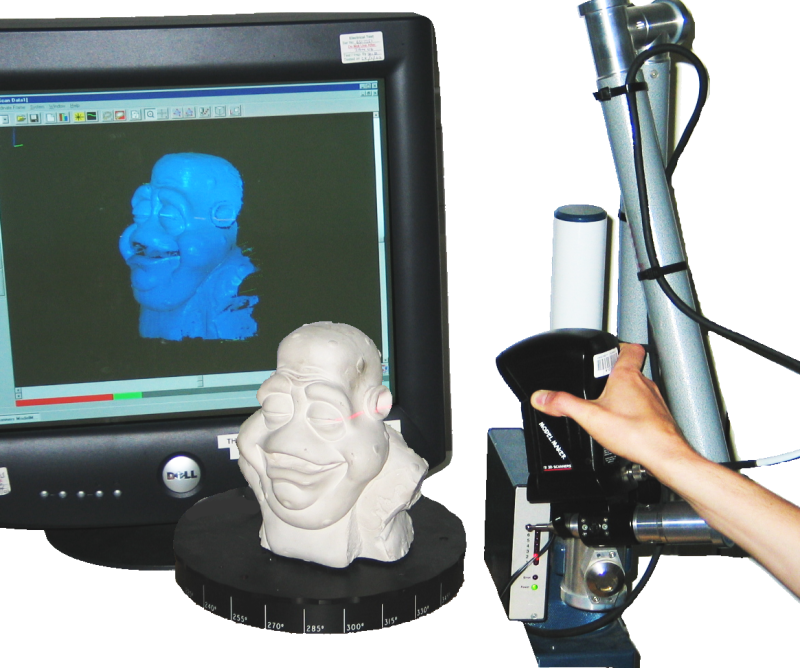
\includegraphics[height=3.8cm]{../images/modelmaker_dino} &
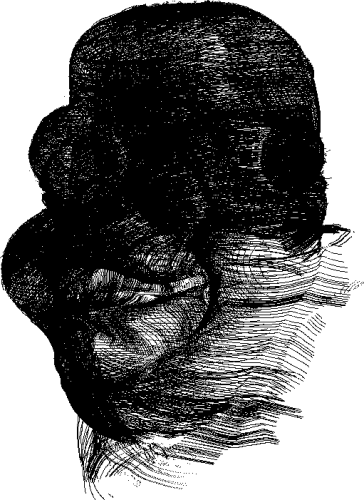
\includegraphics[height=3.8cm]{../images/scandata} &
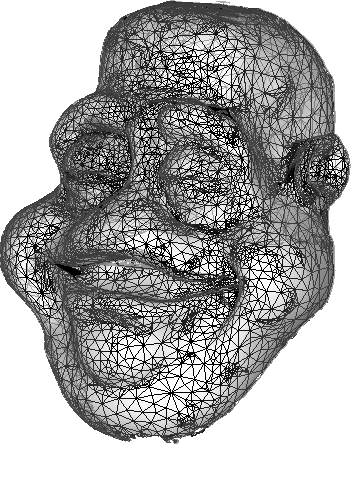
\includegraphics[height=3.8cm]{../images/decimated_wireframe} &
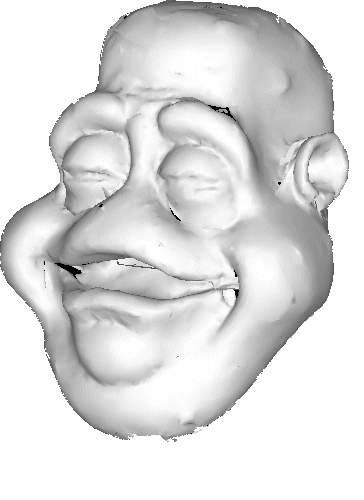
\includegraphics[height=3.8cm]{../images/decimated_smoothshaded} \\
{\it(a)} & {\it(b)} & {\it(c)} & {\it(d)}
\end{tabular}
\caption[Surface Data Capture]{\label{fig:modelmaker} Surface Data Capture. (a) Data is captured with a laser range scanner. (b) Raw scan data points. (c) A simplified polygonal mesh generated from the scan data. (d) A smoothly shaded view of the polygon mesh.}
\end{center}
\end{figure}
The first stage in the process is the capturing of dense surface data from the object to be modelled. In our case this is carried out using a hand-held laser range sensor, the ModelMaker system from \citet{3DScanners} (see figure \ref{fig:modelmaker}a). The operator moves the scanner over the surface in a straight line, capturing a strip of surface measurements, shown in figure \ref{fig:modelmaker}b, which are then converted into a triangle mesh. As the operator will typically scan a number of strips, a number of polygon meshes will be created. These are then fused together using the method proposed by \citet{Hilton96b}, described above in section \ref{sec:litreview:reconstruction:implicit}. The result of this process is a single, very dense, high-resolution triangle mesh with the same geometry as the original object, a simplified version of which is shown in figure \ref{fig:modelmaker}c. This will be used to form the high-resolution detail layer of our model.

\subsection{\label{sec:scandata:creation:control}Control Layer Creation}
Once we have scanned the surface data which will form the detail layer of our model, we must obtain a control layer mesh. There are a number of properties we require in this mesh, both aesthetic and geometric. Firstly, it should follow the geometry of the detail layer closely. Secondly, it should be of a suitable form for animation; i.e. it should be sufficiently detailed and structured in the right way that all animation we wish to perform is possible. Thirdly, it should be structured in such a way as to minimise the collapse of its normal volumes; this will allow us to define an effective mapping between the layers. We may also wish to enforce a maximum error between the two surfaces, again to create a good mapping. We may also require the mapping from the detail to control layer to be injective, for reasons which will be discussed in chapter \ref{sec:dispmapcreation}.

\begin{figure}
\begin{center}
\begin{tabular}{ccc}
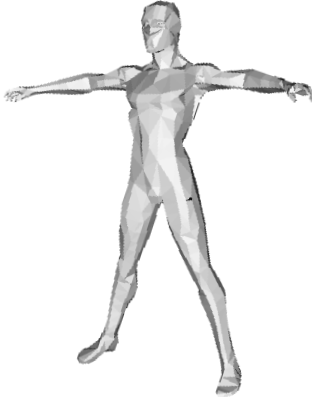
\includegraphics[width=3.5cm]{../images/control_stock} &
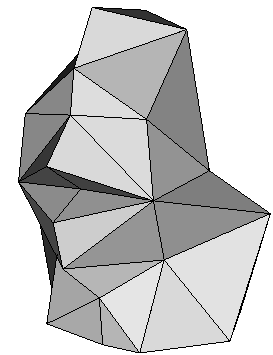
\includegraphics[width=3.5cm]{../images/dinohead_control} &
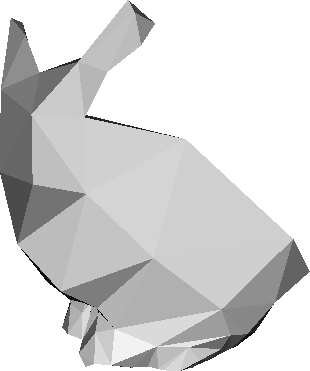
\includegraphics[width=3.5cm]{../images/control_automatic} \\
{\it(a)} & {\it(b)} & {\it(c)}
\end{tabular}
\caption[Control Layer Meshes]{\label{fig:controlmodels} Examples of Control Layer Mesh creation methods (a) Stock model. (b) Interactive creation. (c) Automatic decimation.}
\end{center}
\end{figure}

A control layer mesh can be obtained in a number of different ways. Firstly, it can be a stock model with the same gross shape as the detail layer, and with a structure appropriate for animation, as shown in figure \ref{fig:controlmodels}a. Examples include standard models from \citet{Viewpoint}. 

Alternatively, the control layer can be generated directly from the detail layer. This has the advantage that the control layer is guaranteed to fit the detail layer precisely, and that the error between the two layers will generally be small. The control layer can be generated using either interactive (figure \ref{fig:controlmodels}b) or automatic (figure \ref{fig:controlmodels}c) techniques. Both have their advantages and disadvantages, as we discuss below.

\subsubsection{\label{sec:scandata:creation:control:interactive}Interactive Methods}
\begin{figure}
\begin{center}
\begin{tabular}{cccc}
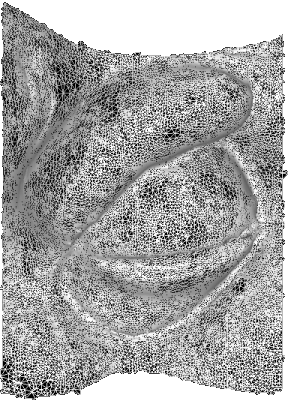
\includegraphics[width=3.18cm]{../images/eye_dense} &
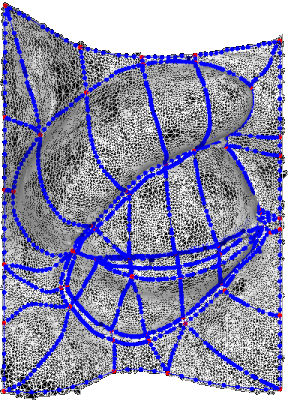
\includegraphics[width=3.18cm]{../images/eye_polylines} &
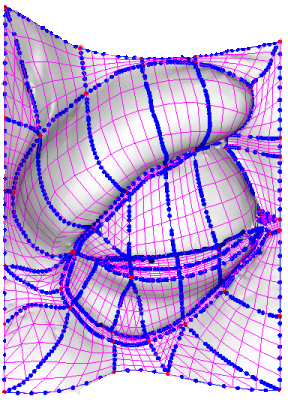
\includegraphics[width=3.18cm]{../images/eye_generate} &
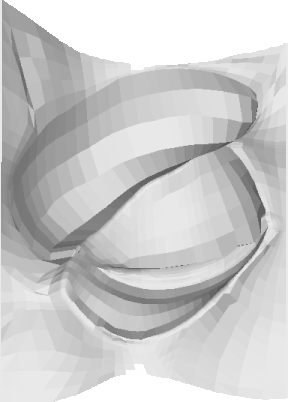
\includegraphics[width=3.18cm]{../images/eye_remesh} \\
{\it(a)} & {\it(b)} & {\it(c)} & {\it(d)}
\end{tabular}
\caption[The 3D Scanners Remesh re-modelling process]{\label{fig:remesh}The 3D Scanners Remesh re-modelling process. (a) The scan data is reconstructed into a polygonal mesh. (b) Lines are drawn onto this mesh, splitting the surface into patches. (c) The patches are subdivided equally, with the subdivisions following the surface, which then are used to create a remodelled mesh (d).}
\end{center}
\end{figure}
Using appropriate software, it is possible to interactively create an appropriate control layer, by creating a lower-resolution version of the detail layer. One technique for doing this is demonstrated in figure \ref{fig:remesh}, which shows the process using the Remesh software package from \citet{3DScanners}. 

Once the dense mesh has been scanned into the system, shown in figure \ref{fig:remesh}a, a trained operator can interactively draw {\it polylines} across the surface of the mesh. These are connected to form triangular or quadrilateral patches (see figure \ref{fig:remesh}b), which can then be subdivided by an appropriate factor (see figure \ref{fig:remesh}c). The subdivided patches define the topology of the control mesh, and the geometry is sampled directly from the scanned data. This technique is basically a controlled resampling of the scan data,  which puts the density and location of the sampling points under the control of the modeller.

Interactive control layer generation has the advantage that it is possible for a human operator to design a control layer structure suitable for animation. Polylines can be placed along the natural lines of the detail layer, and more patches can be placed in areas where more mesh flexibility is required. However, the creation of the control mesh takes time, and it is impossible to enforce geometric constraints such as those mentioned above. We would like to keep user interaction to a minimum, so an alternative approach is to use an automatic method of control layer creation.

\subsubsection{\label{sec:scandata:creation:control:automatic}Automatic Methods}

As an alternative to interactive methods, automated methods can be used to generate the control layer mesh. Such methods have an advantage in that we can guarantee that the resulting mesh will satisfy the geometric conditions described above.

Automatic generation methods can guarantee these conditions by carrying out a controlled decimation of the detail layer, using the conditions as a part of the decimation process. While it is difficult to enforce subjective constraints that are easily done by a trained operator using interactive methods, surface properties such as curvature could also be taken into consideration during the decimation process, in order to create a more appropriate mesh structure.

\citet{Collins02} have defined an automatic decimation method based on the work presented herein, which guarantees an injective mapping between the high and low resolution meshes. This method is of particular interest to us, as we require an injective mapping in order to carry out the displacement mapping technique described below in chapter \ref{sec:dispmapcreation}.

This method defines a test which determines if an injective mapping is possible, by comparing the normals of the high and low resolution meshes. If the dot product of these normals is greater than zero, the surfaces are similarly oriented. As long as this condition holds true across the surfaces of both meshes, then an injective mapping is guaranteed. The decimation is performed by collapsing edges in the high-resolution mesh and testing after each collapse that the orientation condition is preserved. The comparison uses the interpolated normal of the low-resolution mesh, as described above for normal volumes. The algorithm can reduce polygon counts by around 99\%, while guaranteeing an injective mapping.

The major problem with this approach is that it will not normally produce models that are suitable for animation. The decimated control mesh is likely to be as unstructured as the detail mesh from which it was generated.

\subsubsection{\label{sec:scandata:creation:control:semiautomatic}Semi-Automatic Methods}

The best results may, in fact, be obtained from a fusion of the two approaches discussed above. A trained operator could create a mesh with a structure suitable for animation, which an automatic process could then refine to enforce the desired geometric properties. This approach is worthy of further research, but is not covered in this thesis.

\subsection{\label{sec:scandata:creation:skeletalmapping}Control Layer to Skeleton Mapping}

Once the control layer has been created, we can fit a skeleton inside it as described in section \ref{sec:skeletalanim:fitting} and perform the mapping between these two layers. If the control and detail layers have radically different geometries (for instance a human body in a different pose), which is possible if a stock control layer is used, we fit the same skeleton structure inside the detail layer. The difference in pose between the skeletons in then used to deform the control layer to fit the detail layer before mapping occurs.

\subsection{\label{sec:scandata:creation:mapping}Detail to Control Layer Mapping}

\begin{figure}
\begin{center}
\begin{tabular}{cc}
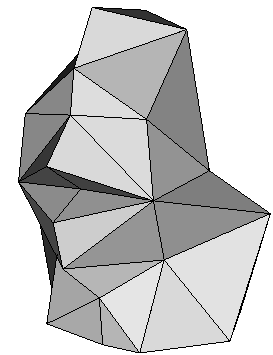
\includegraphics[width=6cm]{../images/dinohead_control} &
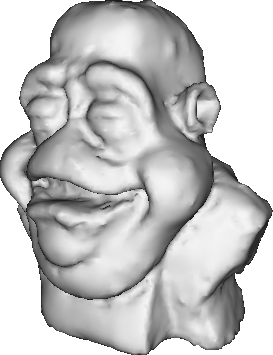
\includegraphics[width=6cm]{../images/dinohead_detail} \\
{\it (a)} & {\it (b)} \\
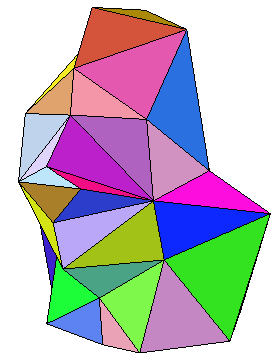
\includegraphics[width=6cm]{../images/dinohead_control_colour} &
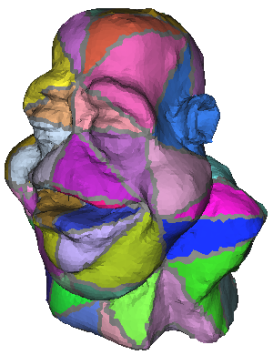
\includegraphics[width=6cm]{../images/dinohead_mapflat} \\
{\it (c)} & {\it (d)}
\end{tabular}
\caption[Detail layer mapping]{\label{fig:detailmapping} Detail Layer Mapping. (a) Control mesh. (b) Detail Layer. (c) Coloured control mesh. (d) Mapping of detail layer points to control mesh triangles. The triangles on the model shown in (d) are coloured according to the triangle in (c) that their vertices map to. Triangles with vertices that map to more than one control mesh triangle are coloured grey. }
\end{center}
\end{figure}
We must then calculate the mapping between the control and detail layers. Using the method described in section \ref{sec:scandata:pointtosurface}, we perform an exhaustive search, attempting to map each detail layer point to each control layer triangle in turn\footnote{This search could be constrained by taking point and triangle adjacency information into account, but this is not included in our current method.}. A valid result should only be obtained for one control triangle. In the case where more than one valid result is found, for instance in areas of high curvature where normal volumes intersect, the result with the lowest value for $d$ is chosen. This simple distance criterion may not always give the correct mapping however, so other information should also be considered, for instance surface orientation. This issue should also be taken into account during control mesh creation, where it could be checked for and avoided during the automatic decimation process. If $v_d$ represents the number of detail layer vertices, and $t_c$ the number of control layer triangles, the mapping algorithm for a complete mesh has order $O(v_d t_c)$.

Once all detail layer points have been mapped, the original detail layer data can be discarded. The geometry of the detail layer can then be rebuilt from the mapping results as shown in figure \ref{fig:detailmapping}d. The faces of the model are coloured according to which control layer triangle they map to - the coloured control layer is shown in figure \ref{fig:detailmapping}c. Detail layer triangles which have vertices mapping to different control layer triangles are coloured grey.

\subsection{\label{sec:scandata:creation:lmtool}LMTool Interface}

\begin{figure}
\begin{center}
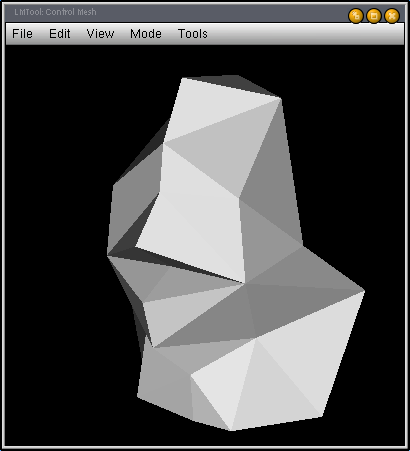
\includegraphics[width=3.5cm]{../images/lmtool_control}
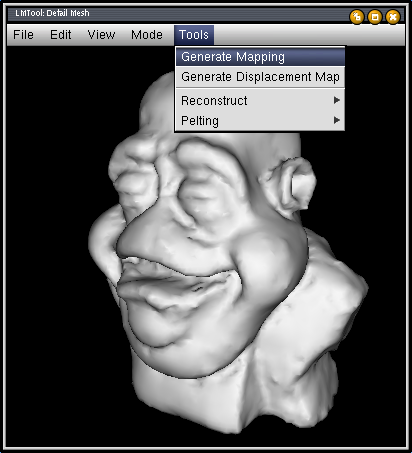
\includegraphics[width=3.5cm]{../images/lmtool_detail}
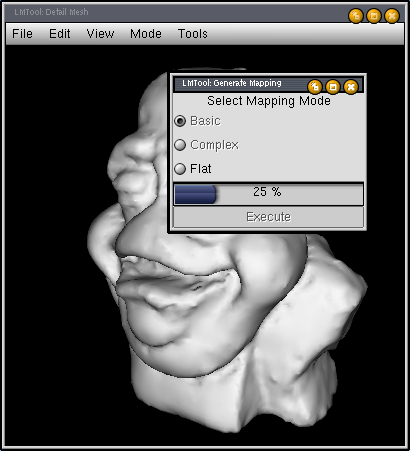
\includegraphics[width=3.5cm]{../images/lmtool_mapdialog}
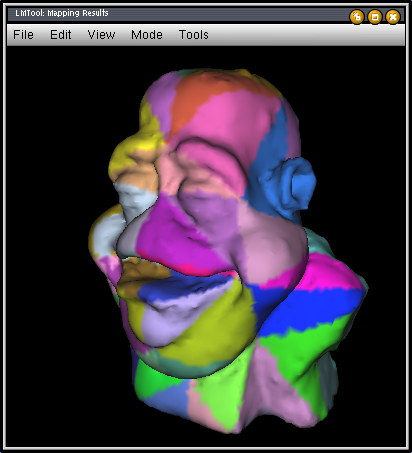
\includegraphics[width=3.5cm]{../images/lmtool_mapping}
\caption[LMTool Application Interface.]{\label{fig:lmtool} LMTool Application Interface. The screenshots show the process of loading a control and detail layer, then performing the mapping between the two.}
\end{center}
\end{figure}

During this research, a graphical software application was created to assist in the creation and manipulation of our layered models, called {\it LMTool}. It was developed on a Linux platform, and based on both the AMMA software library \cite{AMMA} created by the CVSSP, and OpenGL \cite{OpenGL} for the 3D graphical display.

LMTool has many functions within it, most of which will be discussed later on in this thesis. At this stage, we are simply interested in the process of creating layered models from a pair of polygon meshes. Upon starting the application, two polygon meshes are loaded. The first is the control layer, shown in figure \ref{fig:lmtool}a. The second is the scanned surface data, shown in figure \ref{fig:lmtool}b, which will be used to create the detail layer of our model. To perform the mapping, a menu option is selected and a dialog is displayed. This dialog allows the user to choose which mapping algorithm should be used\footnote{Various experimental mapping algorithms were used throughout the course of this thesis. All were minor variations on the final version presented here, and will not be discussed further herein.}. Upon pressing ``Execute'', the application then performs the point-to-surface mapping process described in section \ref{sec:scandata:pointtosurface}. The results are then displayed in the window, with the mesh coloured as described in figure \ref{fig:detailmapping}.

LMTool does not presently include skeletal animation capabilities, so is limited to the execution of the mapping process and the rebuilding of mapped detail layers. The control mesh can, however, be manipulated manually within the tool, allowing some rudimentary animation to be carried out. The user can select vertices on the control mesh and drag them around in the window. Some animation using this technique will be shown in section \ref{sec:scandata:results} below.

\section{\label{sec:scandata:results}Results}

\begin{table}
\begin{center}
\begin{tabular}{c|c|c|c|c|c} 
Model & & Cubehead & Monster & Horse & Bunny \\
\hline
			& Vertices & 2215 & 15045  & 48485 & 34876 \\
\raisebox{1.5ex}{Detail}& Triangles & 4042 & 30086  & 96966 & 69535 \\
\hline
  	& Method & Stock & Interactive & Automatic & Automatic \\
Control & Vertices & 8 & 32  & 407 & 487 \\
  	& Triangles & 12 & 60  & 810 & 757 \\
\hline
\end{tabular}
\caption[Model Statistics]{\label{tbl:models} Model Statistics. }
\end{center}
\end{table}

We have tested our mapping algorithm on a number of different models, which are shown in figure \ref{fig:models}. Statistics for the models are shown in table \ref{tbl:models}. The bottom row of the figure shows the results of the mapping for each model. The geometry of the mapped models is rebuilt from the mapped detail layer, but is identical to the original detail layer mesh in every way.

\begin{figure}
\begin{center}
\begin{tabular}{cccc}
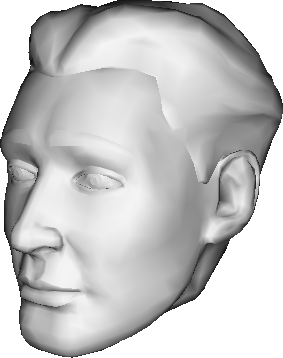
\includegraphics[height=3cm]{../images/cubehead_detail} &
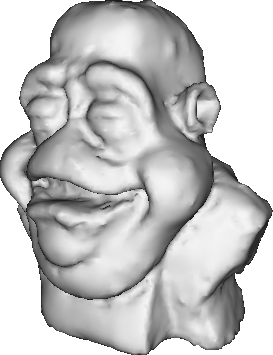
\includegraphics[height=3cm]{../images/dinohead_detail} &
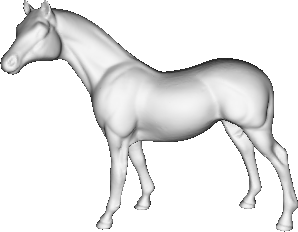
\includegraphics[height=3cm]{../images/horse_detail} &
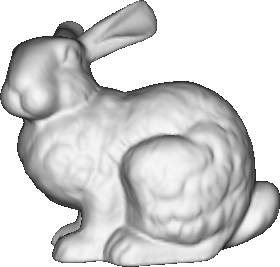
\includegraphics[height=3cm]{../images/bunny_detail} \\
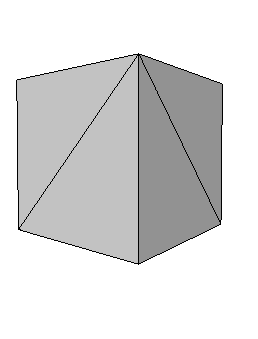
\includegraphics[height=3cm]{../images/cubehead_control} &
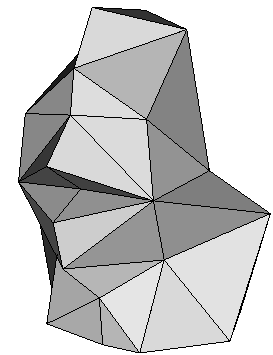
\includegraphics[height=3cm]{../images/dinohead_control} &
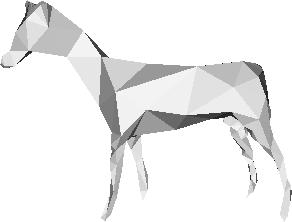
\includegraphics[height=3cm]{../images/horse_control} &
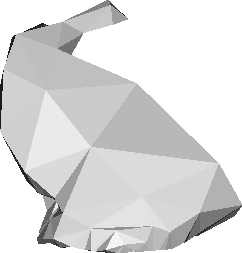
\includegraphics[height=3cm]{../images/bunny_control} \\
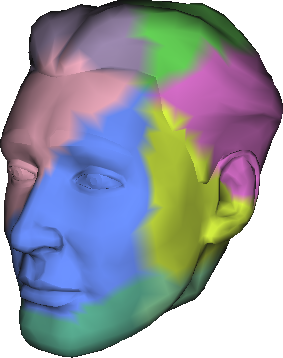
\includegraphics[height=3cm]{../images/cubehead_mapsmooth} &
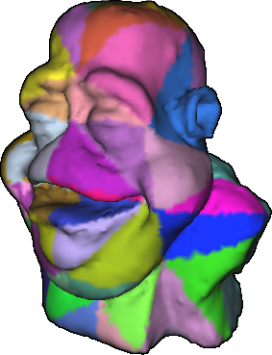
\includegraphics[height=3cm]{../images/dinohead_mapsmooth} &
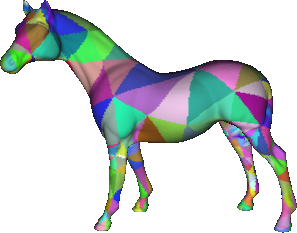
\includegraphics[height=3cm]{../images/horse_mapsmooth} &
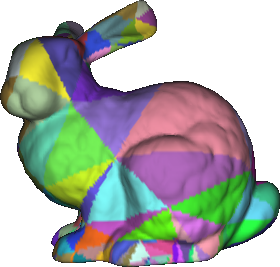
\includegraphics[height=3cm]{../images/bunny_mapsmooth} \\
{\it (a)} & {\it (b)} & {\it (c)} & {\it (d)} 
\end{tabular}
\caption[Test Models]{\label{fig:models} Test Models. (a) Cubehead. (b) Monster. (c) Horse. (d) Bunny. The top row shows the detail layer mesh, while the middle row shows the control layer. The bottom row shows the reconstructed mapped detail layers, coloured as explained in figure \ref{fig:detailmapping}. }
\end{center}
\end{figure}

\subsection{\label{sec:scandata:results:animation} Animation}

\begin{figure}
\begin{center}
\begin{tabular}{ccc}
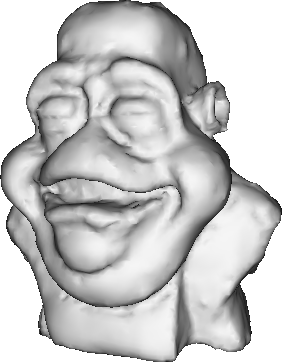
\includegraphics[width=3cm]{../images/mapanim_1} &
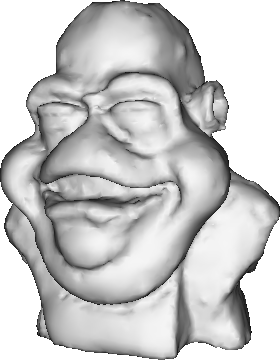
\includegraphics[width=3cm]{../images/mapanim_2} &
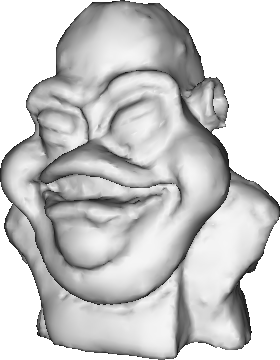
\includegraphics[width=3cm]{../images/mapanim_3} \\
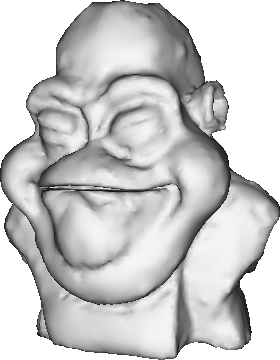
\includegraphics[width=3cm]{../images/mapanim_4} &
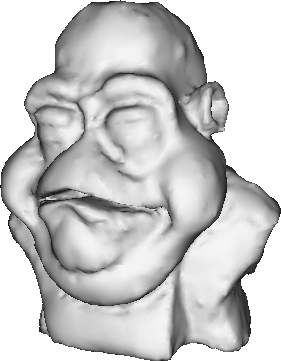
\includegraphics[width=3cm]{../images/mapanim_5} &
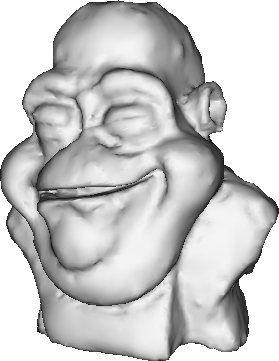
\includegraphics[width=3cm]{../images/mapanim_6} \\
& (a) &
\end{tabular}
\begin{tabular}{cc}
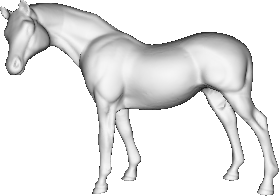
\includegraphics[width=4cm]{../images/horse_mapanim2} &
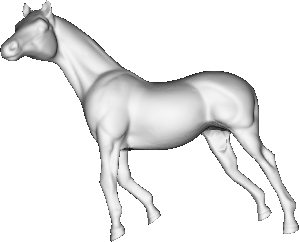
\includegraphics[width=4cm]{../images/horse_mapanim3} \\
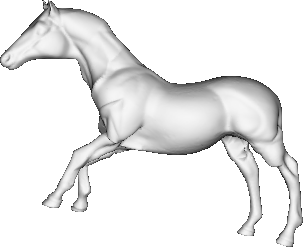
\includegraphics[width=4cm]{../images/horse_mapanim4} &
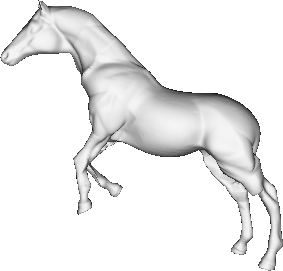
\includegraphics[width=4cm]{../images/horse_mapanim5} \\
\multicolumn{2}{c}{(b)}
\end{tabular}
\caption[Detail Layer Animation]{\label{fig:detailanim} Detail Layer Animation. (a) Facial animation of the Monster head, performed by direct manipulation of control mesh vertices. (b) Horse animation, performed by animation of the control mesh in 3D Studio MAX.}
\end{center}
\end{figure}

Figure \ref{fig:detailanim} shows animation of the mapped detail layer, for the Monster and Horse models. By manipulating the control layer mesh, we can perform animation of the complex datasets that make up the detail layer. As the control mesh for a model is animated, the rebuilt detail layer deforms with it. As the normal volumes of the control layer stretch, the normals within them are smoothly interpolated, and the detail layer stretches smoothly across the surface of the polygon.

\section{\label{sec:scandata:conclusion}Conclusion}

In this chapter, we have presented a method of animating densely scanned surface data based on animation of a lightweight control mesh. The method enables animators to use a simplified version of the scanned data for realtime animation planning, which can then be used to automatically perform the same animation on the dense surface in an offline rendering process. Once a suitable control mesh and skeleton structure have been created, the mapping process itself is fully automatic.

The main limitation of this animation method is that it requires us to animate and recalculate the entire detail layer surface, which may consist of a very large number of polygons. This is not a problem for high-quality offline production, which can take as long as is necessary to obtain a realistic result, but it is impossible to use for interactive applications. Therefore, in the next chapter, we introduce an alternative representation of the detail layer surface which will enable us to reconstruct the detail layer surface to an arbitrary levels of detail.

